\documentclass[12pt]{standalone}
\usepackage[utf8]{inputenc}
\usepackage[T1]{fontenc}
\usepackage{times}
\usepackage{amsmath,amssymb}
\usepackage[dvipsnames,svgnames]{xcolor}
\usepackage{tikz}
\usetikzlibrary{calc, positioning, arrows.meta}
\definecolor{dmrsfill}{HTML}{CDE2FB}
\definecolor{winblue}{HTML}{0D366B}
\definecolor{inksec}{HTML}{52514E}
\definecolor{interf}{HTML}{C0504D}
% O que chega à DU 3 na primeira iteração (exemplo da Figura rn_blocos, C = 4).
% Pré-processamento: b_0 = soma de W_c^0 n_c^i de todas as DUs (Algoritmo 3 de Zhao et al. 2025).
% Cada DU troca a sua parcela antiga pela nova (Eq. eq:b_update). A DU 3 recebe b_{2,i}, subtrai a
% sua parcela antiga (Eq. eq:bcd_update) e multiplica pelas suas amostras.
% Conta: (1/N) sum_i W_j n_j^i (n_3^i)^H = W_j R_j3, com R_j3 = (1/N) sum_i n_j^i (n_3^i)^H.
\newcommand{\novo}[1]{\textcolor{winblue}{#1}}
\newcommand{\velho}[1]{\textcolor{inksec}{#1}}
\begin{document}
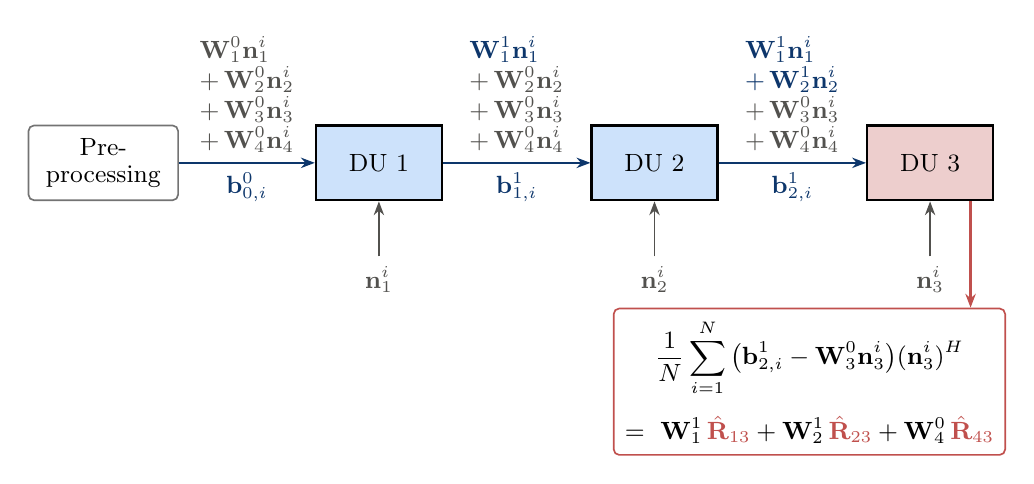
\begin{tikzpicture}[font=\fontsize{9}{10.8}\selectfont, >={Stealth[length=5pt]}]
\tikzset{du/.style={draw, line width=0.8pt, fill=dmrsfill, minimum width=1.6cm, minimum height=0.95cm, align=center},
         dur/.style={draw, line width=0.8pt, fill=interf!28, minimum width=1.6cm, minimum height=0.95cm, align=center},
         pre/.style={draw=black!55, line width=0.6pt, rounded corners=2pt, minimum width=1.9cm, minimum height=0.95cm, align=center}}
\node[pre] (p)  at (0,0)    {Pre-\\[-1pt]processing};
\node[du]  (d1) at (3.5,0)  {DU 1};
\node[du]  (d2) at (7.0,0)  {DU 2};
\node[dur] (d3) at (10.5,0) {DU 3};
% b ao longo da cadeia na iteração 1: cada DU troca a sua parcela
\draw[->, winblue, line width=0.8pt] (p) -- node[above, align=left] {%
  \velho{$\mathbf W_1^0\mathbf n_1^i$}\\\velho{$+\,\mathbf W_2^0\mathbf n_2^i$}\\\velho{$+\,\mathbf W_3^0\mathbf n_3^i$}\\\velho{$+\,\mathbf W_4^0\mathbf n_4^i$}} (d1);
\draw[->, winblue, line width=0.8pt] (d1) -- node[above, align=left] {%
  \novo{$\mathbf W_1^1\mathbf n_1^i$}\\\velho{$+\,\mathbf W_2^0\mathbf n_2^i$}\\\velho{$+\,\mathbf W_3^0\mathbf n_3^i$}\\\velho{$+\,\mathbf W_4^0\mathbf n_4^i$}} (d2);
\draw[->, winblue, line width=0.8pt] (d2) -- node[above, align=left] {%
  \novo{$\mathbf W_1^1\mathbf n_1^i$}\\\novo{$+\,\mathbf W_2^1\mathbf n_2^i$}\\\velho{$+\,\mathbf W_3^0\mathbf n_3^i$}\\\velho{$+\,\mathbf W_4^0\mathbf n_4^i$}} (d3);
\foreach \a/\b/\l in {p/d1/{\mathbf b_{0,i}^0}, d1/d2/{\mathbf b_{1,i}^1}, d2/d3/{\mathbf b_{2,i}^1}}
  \node[winblue, below] at ($(\a.east)!0.5!(\b.west)$) {$\l$};
% amostras locais
\foreach \n/\c in {d1/1, d2/2, d3/3}
  \draw[->, inksec, line width=0.6pt] ($(\n.south)+(0,-0.7)$) node[below] {$\mathbf n_{\c}^i$} -- (\n.south);
% o que a DU 3 calcula
\node[draw=interf, line width=0.6pt, rounded corners=2pt, align=center, inner sep=4pt, anchor=north east] (res) at ($(d3.south east)+(0.15,-1.35)$)
  {$\dfrac{1}{N}\displaystyle\sum_{i=1}^{N}\big(\mathbf b_{2,i}^1 - \mathbf W_3^0\mathbf n_3^i\big)(\mathbf n_3^i)^H$\\[6pt]
   $=\ \mathbf W_1^1\,\textcolor{interf}{\hat{\mathbf R}_{13}} + \mathbf W_2^1\,\textcolor{interf}{\hat{\mathbf R}_{23}} + \mathbf W_4^0\,\textcolor{interf}{\hat{\mathbf R}_{43}}$};
\coordinate (sai) at ($(d3.south east)+(-0.3,0)$);
\draw[->, interf, line width=0.8pt] (sai) -- (sai |- res.north);
\end{tikzpicture}
\end{document}
